\chapter{Introduzione}

\section{Perché Agenti Intelligenti?}

\paragraph{La storia della computazione è stata definità da 5 trends:}


\begin{itemize}
  \item \fancyglitter{Ubiquità}. 
  \item \fancyglitter{Interconnessione}. 
  \item \fancyglitter{Intelligenza}. 
  \item \fancyglitter{Delega}. 
  \item \fancyglitter{Human-orientation}.
\end{itemize}

\paragraph{Ubiquità:}

\begin{itemize}
  \item La continua riduzione dei costi di elaborazione ha permesso di introdurre capacità di elaborazione in luoghi e dispositivi che una volta sarebbero stati antieconomici. 
  \item Ma mano che la capacità di elaborazione si diffonde, elementi sofisticati e intelligenti diventano onnipresenti.
\end{itemize}

\paragraph{Interconnessione:}

\begin{itemize}
  \item I sistemi informatici, attualmente, non esistono più da soli, ma sono collegati in rete in grandi sistemi distribuiti.
\item Per esempio internet. 
\item Alcuni ricercatori stanno proponendo modelli teorici che ritraggono l'informatica principalmente come un processo di interazione.
\end{itemize}

\paragraph{Intelligenza e Delega:}

\begin{itemize}
  \item La complessità dei compiti che siamo capaci di automatizzare e delegare ai computer è cresciuta costantemente. 
  \item Viene dato più controllo ai computer: 
    \begin{itemize}
      \item \textit{Fly-by wire aircraft}. 
      \item \textit{Fly-by-wire cars}.
    \end{itemize}
\end{itemize}

\paragraph{Human-orientation:}

\begin{itemize}
  \item CI si sposta da una vista orientata alla macchina e alla programmazione verso una visione a metafore e concetti più vicine alla comprensione umana. 
  \item I programmatori concettualizzano e realizzano software in termini di livello superiore, più orientato all'uomo, \fancyglitter{astrazioni}.
\end{itemize}

\nt{Delega e intelligenza implicano la necessità di costruire sistemi informatici in grado di agire efficacemente.}

\paragraph{Questo implica:}

\begin{itemize}
  \item La capacità di agire dei sistemi informatici \fancyglitter{in modo indipendente}\footnote{Un oggetto fa qualcosa perché la deve fare, un agente fa qualcosa perché la vuole fare. Hey non avevo idea di essere diventat un oggetto quando mi sono iscritt all'università.}. 
  \item La capacità dei sistemi informatici di agire in un modo che \fancyglitter{rappresentino nel migliore dei modi i nostri interessi} durante l'interazione con altri esseri umani o sistemi.
  \item Interconnessione e distribuzione portano a sistemi che possono \fancyglitter{cooperare} e \fancyglitter{raggiungere accordi}, \fancyglitter{agreements} o \fancyglitter{competere} con altri sistemi che hanno interessi diversi.
  \item Tutto ciò porta alla nascita di un nuovo campo dell'informatica: \fancyglitter{sistemi multiagente}.
\end{itemize}

\subsection{Agenti e Sistemi Multiagente}

\dfn{Agente}{
  Un agente è un sistema di compilazione, un sistema informatico, capace di agire in modo indipendente per conto di un utente o proprietario (capendo cosa deve essere fatto per soddisfare gli obiettivi di progettazione, piuttosto che essere costantemente informato).
}

\dfn{Sistema Multiagente}{
  Un sistema multiagente (MAS) consiste in una serie di agenti, che interagiscono l'uno con l'altro. Nel caso più generale, gli agenti agiscono per conto di utenti con differenti obiettivi e mtivazioni.
}

\nt{per interagire con successo, richiedono la capacità di \fancyglitter{cooperare}, \fancyglitter{coordinarsi} e \fancyglitter{negoziare} tra loro.}

\paragraph{Un sistema multiagente risponde a queste domande:}

\begin{itemize}
  \item Come può emergere la cooperazione in società composte da agenti \textit{self-interested}?
  \item Quali tipi di linguaggi possono essere utilizzati dagli agenti per comunicare?
  \item Come possono gli agenti \textit{self-interested} riconoscere conflitti? E come possono raggiungere accordi?
  \item Come possono gli agenti autonomi coordinare le proprie attività in modo da raggiungere cooperativamente gli obiettivi?
\end{itemize}

\paragraph{Ma soprattutto:}

\begin{itemize}
  \item Come possiamo creare agenti capaci di agire in modo indipendente, autonomo, in modo che possano svolgere con successo i compiti che gli deleghiamo?
  \item Come possiamo creare agenti capaci di interagire con altri agenti con il fine di portare a termine con successo i compiti delegati, soprattutto quando non si può presumere che gli altri agenti condividano gli stessi interessi e obiettivi?
\end{itemize}

\clm{}{}{
  \begin{itemize}
    \item Il primo caso è un problema di progettazione/design di un agente. 
    \item Il secondo caso è un problema di progettazione/design di società di agenti.
  \end{itemize}
}

\subsection{Approccio Interdisciplinare}

\paragraph{Il campo dei sistemi multiagente è influenzato e ispirato da molti altri campi:}

\begin{itemize}
  \item Economia. 
  \item Filosofia. 
  \item Teoria dei giochi. 
  \item Logica. 
  \item Ecologia. 
  \item Scienze sociali.
\end{itemize}

\nt{Questo è sia un punto di forza (perché ci sono molte idee diverse) sia un punto di debolezza (perché ci sono molte idee diverse lol).}

\qs{}{Non è solo AI?}

\begin{itemize}
  \item Non abbiamo bisogno di risolvere tutti i problemi di intelligenza artificiale per costruire agenti utili. 
  \item L'AI classica ignorava gli aspetti sociali dell'agire.
\end{itemize}

\qs{}{Non è solo economia/teoria dei giochi?}

\begin{itemize}
  \item Nella misura in cui la teoria dei giochi fornisce descrizione di concetti, non sempre ci dice come calcolare soluzioni. 
  \item Alcune assunzioni in economia/teoria dei giochi potrebbero non essere valide o utili nella costruzione di agenti artificiali.
\end{itemize}

\qs{}{Non sono solo scienze sociali?}

\begin{itemize}
  \item Possiamo trarre spunti dallo studio di società umane, ma non ci sono particolari motivi per credere che le società artificiali siano costruite allo stesso modo\footnote{Effettivamente sarebbe raccapricciante se gli agenti cominciassero a uccidersi a vicenda per questioni triviali.}. 
  \item Si trae ispirazione, ma non si assume a prescindere.
\end{itemize}
\pagebreak

\section{Cosa si Intende per Agenti Intelligenti?}

Ricordiamo che un agente è un sistema di computazione capace di agire \fancyglitter{autonomamente} in un qualche \fancyglitter{ambiente} con il fine di raggiungere gli \fancyglitter{obiettivi} per cui è progettato.

\nt{La caratteristica principale degli agenti e la loro autonomia.}

  \begin{figure}[h]
    \centering
    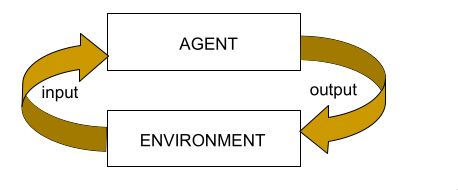
\includegraphics[scale=0.7]{01/ae.png}
    \caption{Agente che interagisce con l'ambiente.}
    \label{fig:ae}

  \end{figure}

\nt{In figura \ref{fig:ae} il fatto che l'agente e l'ambiente sono disegnati con due rettangoli identici non è casuale: sono due elementi alla pari.}

\ex{Agenti}{
  \begin{center}
    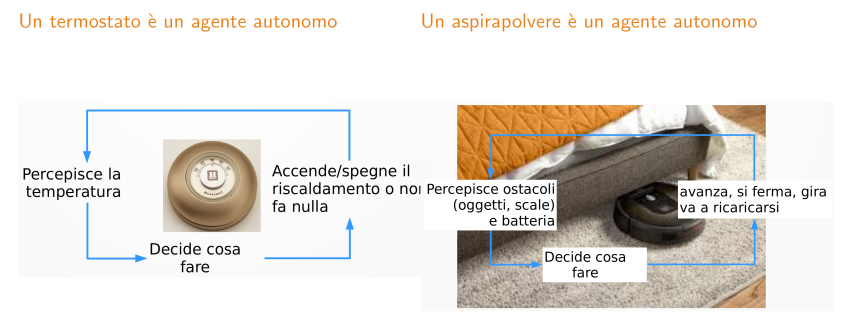
\includegraphics[scale=0.55]{01/ta.png}
  \end{center}
}

\paragraph{Autonomia e controllabilità:}

\begin{itemize}
  \item Al di fuori della comunità AI, gli agenti autonomi intelligenti sono percepiti come entità consapevoli di sé, incontrollabili, la cui autonomia emerge come proprietà "extra-programma". 
  \item Un agente può prendere iniziative che non sono incluse fin dall'inizio nel suo programma.
\end{itemize}
\pagebreak
\subsection{Test di Turing}

\paragraph{Il test di Turing:}

\begin{itemize}
  \item Una persona o un computer sono nascosti a un investigatore (fig. \ref{fig:Turing}).
  \begin{figure}[h]
    \centering
    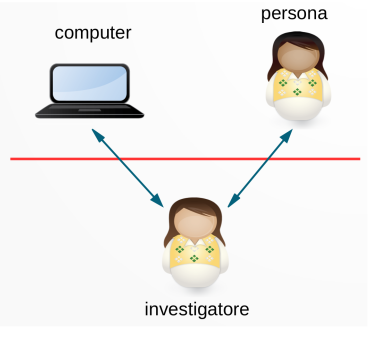
\includegraphics[scale=0.4]{01/turing1.png}
    \caption{Rappresentazione del test di Turing.}
    \label{fig:Turing}
  \end{figure}
   \item Interazione:
     \begin{itemize}
      \item L'investigatore pone domande scritte. 
      \item L'entità nascosta fornisce risposte scritte. 
      \item L'investigatore deve capire se dall'altra parte c'è un computer o una persona. Se all'altra parte c'è un computer e l'investigatore non riesce a distinguerlo allora il computer si può dire \fancyglitter{intelligente}.
     \end{itemize}
   \item Basta produrre gli output attesi per dire che vi è comprensione? (fig. \ref{fig:Turing2})
  \begin{figure}[h]
    \centering
    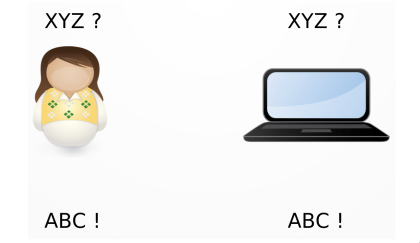
\includegraphics[scale=0.4]{01/turing2.png}
    \caption{Scambio di messaggi.}
    \label{fig:Turing2}
  \end{figure}
\end{itemize}

\paragraph{Esperimento di J. Searle (la stanza cinese):}

\begin{itemize}
  \item Un computer, programmato per rispondere con certi ideogrammi cinesi ad altri ideogrammi cinesi ricevuti in input (fig. \ref{fig:Searle}. L'interlocutore umano che parla in cinese non vede il computer che è chiuso in una stanza. Cosa penserà di chi è nella stanza?
  \begin{figure}[h]
    \centering
    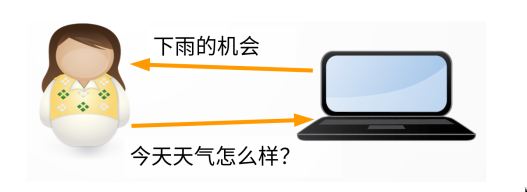
\includegraphics[scale=0.4]{01/searle1.png}
    \caption{Rappresentazione dell'esperimento di Searle.}
    \label{fig:Searle}
  \end{figure}
\item Il computer parla cinese? Lo capisce? 
\item Una persona chiusa in una stanza ha istruzioni per rispondere con certi ideogrammi cinesi in risposta ad altri ideogrammi cinesi (fig. \ref{fig:Searle2}). 
    \begin{figure}[h]
    \centering
    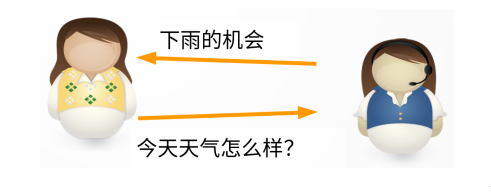
\includegraphics[scale=0.5]{01/searle2.png}
    \caption{Esperimento con una persona.}
    \label{fig:Searle2}
  \end{figure}
\item Scrivere un programma per un computer non è di per sé una condizione sufficiente per implicare l'intenzionalità.
\end{itemize}

\nt{Searle ha scelto il cinese perché voleva considerare una lingua difficile da capire. Per me è skill issue.}

\paragraph{AI:}

\begin{itemize}
  \item \fancyglitter{AI forte}: è possibile riprodurre l'intelligenza umana? Compresa la consapevolezza di sé, l'essere senziente, etc. 
  \item \fancyglitter{AI debole}: esistono modi automatici per risolvere problemi che a un essere umano richiedono intelligenza? Task-oriented, studio del pensiero e del comportamento umano.
\end{itemize}

\subsection{Agenti Intelligenti}

\paragraph{Agenti triviali (non interessanti):}

\begin{itemize}
  \item Termostato. 
  \item UNIX deamon\footnote{Come si permette di dire che il daemon UNIX non è interessante. Probabilmente non ha mai speso il pomeriggio a riaggiustarlo dopo aver rotto un arch install >:(}
\end{itemize}

\paragraph{Un agente intellingente deve eseguire azioni in modo \fancyglitter{flessibile}:}

\begin{itemize}
  \item \fancyglitter{Reattivo}. 
  \item \fancyglitter{Proattivo}. 
  \item \fancyglitter{Sociale}.
\end{itemize}

\clm{}{}{
  \begin{itemize}
    \item Se l'ambiente di un software è statico/fisso non è necessario preocuparsi di esso (e. g. un compilatore, un package manager). 
    \item Nel mondo reale le cose cambiano, le informazioni sono incomplete. 
    \item È necessario considerare la possibilità che l'esecuzione di azioni (istruzioni) non abbia successo, è necessario chiedersi se valga la pena eseguire una certa azione.
  \end{itemize}
}

\dfn{Agente Reattivo}{
  Un agente reattivo è un sistema che mantiene una costante interazione con l'ambiente e risponde ai cambiamenti he occorrono in esso (in tempo perché la risposta sia utile).
}

    \begin{figure}[h]
    \centering
    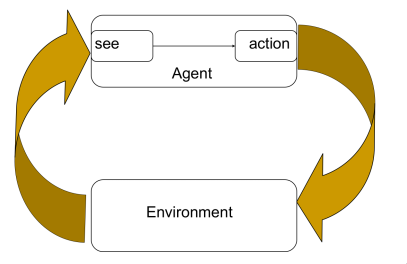
\includegraphics[scale=0.5]{01/agentereattivo.png}
    \caption{Un agente reattivo.}
  \end{figure}

  \nt{Può essere visto come un if then.}

\clm{}{}{
  \begin{itemize}
    \item Reagire a un ambiente è facile, però in generale, si vuole che gli agenti "facciano cose per noi". 
    \item \fancyglitter{Goal directed behaviour}: comportamento guidato dagli obiettivi.
    \item \fancyglitter{Proattività}: generare e tentare di raggiungere gli obiettivi, non solo guidati dagli eventi, ossia \fancyglitter{prendere l'iniziativa}. 
    \item Riconoscere le opportunità.
  \end{itemize}
}

\dfn{Agente Proattivo}{
  Lo stato dell'agente contiene due tipi di conoscenza:
  \begin{itemize}
    \item L'agente necessita di informazioni su come l'ambiente evolve. 
    \item L'agente necessità di informazioni su come le proprie azioni impattano sull'ambiente.
  \end{itemize}
  L'agente necessita di informazioni sull'\newfancyglitter{obiettivo} (goal) in modo che l'agente possa agire per raggiungerlo. Nel farlo l'agente deve essere in grado di lavorare su \newfancyglitter{piani}.
}

\begin{figure}[h]
  \centering
  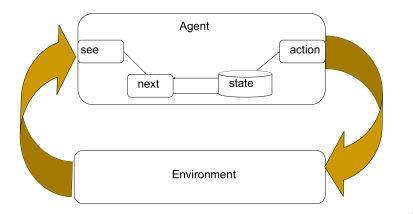
\includegraphics[scale=0.7]{01/proattivo.png}
  \caption{Agente proattivo.}
\end{figure}

\paragraph{Reattivo vs. Proattivo:}

\begin{itemize}
  \item Si desidera che gli agenti siano reattivi e che rispondano ai cambiamenti per tempo. 
  \item Si desidera che gli agenti lavorino in modo sistematico verso obiettivi di lungo termini. 
  \item Queste due considerazioni possono essere in conflitto. 
  \item Progettare un agente che bilanci reattività e proattività è ancora un problema aperto.
\end{itemize}

\clm{}{}{
  \begin{itemize}
    \item Il mondo reale è spesso un ambiente multiagente, per cui non si possono raggiungere i propri obiettivi senza l'aiuto degli altri. 
    \item Alcuni obiettivi possono essere raggiunti solo con la collaborazione di altri. 
    \item Allo stesso modo i sistemi sono immersi in una rete di computer. 
  \end{itemize}
}

\dfn{Abilità Sociale}{
  Per abilità sociale di un agente intelligente si intende l'abilità di interagire con altri agenti (anche umani) attraverso un qualche tipo di \newfancyglitter{linguaggio di comunicazione} (\newfancyglitter{agent-communication language}, \newfancyglitter{ACL}) e cooperare con essi.
}

\qs{}{Agente intelligente o generico programma?}

\dfn{Is it an Agent or just a Program?}{
  Un agente autonomo è un sistema situato in un ambiente che può percepire e agire su di esso nel tempo con il fine di perseguire una propria agenda e così facendo influire nelle successive percezioni.
}

\nt{Secondo questa definizione sia gli esseri umani che i termostati sono agenti autonomi.}

\section{Cenni alla Computazione}

\paragraph{L'ingegneria del software aspira a produrre software di qualità (tramite la \fancyglitter{modularizzazione}):}

\begin{itemize}
  \item Correttezza. 
  \item Robustezza. 
  \item Estensibilità. 
  \item Riusabilità.
\end{itemize}

\nt{Che sono le stesse cose del software \textit{suckless} che è 100\% FOOS, ma ovviamente il prof non ne parla.}

\paragraph{Meyer individua, nei linguaggi di programmazione, tre forze (fig. \ref{fig:meyer}):}

\begin{itemize}
  \item Processo: la CPU fisica, un processo o un thread. 
  \item Azione: operazioni che costituiscono la computazione. 
  \item Oggetto: le strutture dati a cui si applica l'azione.
\end{itemize}

\begin{figure}[h]
  \centering
  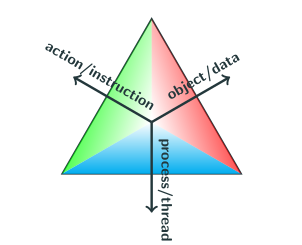
\includegraphics[scale=0.7]{01/meyer.png}
  \caption{Il triangolo di Meyer.}
  \label{fig:meyer}
\end{figure}

\paragraph{Decomposizione funzionale (a dispetto del nome è l'approccio del paradigma imperativo):}

\begin{itemize}
  \item PRO:
    \begin{itemize}
      \item Semplice e intuitivo: si costruisce un sistema con la decomposizione in passi. 
      \item Orientato agli algoritmi: utile quando si ha un solo top goal. 
    \end{itemize}
  \item CONTRO:
    \begin{itemize}
      \item Difficile da mantenere\footnote{Skill issue.}: difficile incorporare nuovi goal. 
      \item Difficilmente scalabile in presenza di dati condivisi e processi concorrenti.
    \end{itemize}
\end{itemize}

\begin{figure}[h]
  \centering
  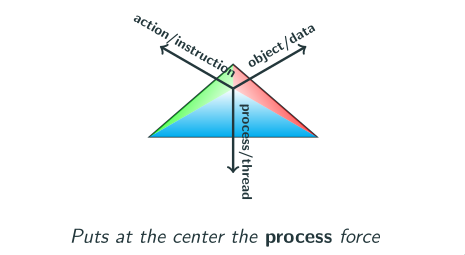
\includegraphics[scale=0.7]{01/func.png}
  \caption{Decomposizione funzionale.}
\end{figure}

\paragraph{Decomposizione orientata agli oggetti:}

\begin{itemize}
  \item PRO: 
    \begin{itemize}
      \item Gli oggetti hanno una vita loro, indipendentemente dal processo che li usa. 
      \item Operazioni sui dati: fornisce azioni per lavorare su essi. 
      \item GLi oggetti sono modelli.
    \end{itemize}
  \item Contro: 
    \begin{itemize}
      \item Gli oggetti sono passivi: un processo esterno prende la decisione su quale azione invocare su un oggetto. 
      \item Non c'è differenza tra uso di un oggetto e gestione di un oggetto. 
      \item Non c'è supporto concettuale alle specifiche di un task. 
    \end{itemize}
\end{itemize}

\begin{figure}[h]
  \centering
  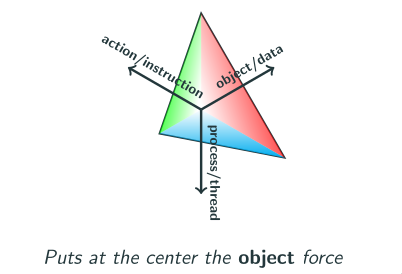
\includegraphics[scale=0.7]{01/oo.png}
  \caption{Decomposizione orientata agli oggetti.}
\end{figure}

\paragraph{Modello ad attori e oggetti attivi:}

\begin{itemize}
  \item Gli attori hanno il proprio thread. 
  \item Il modello degli attori non prende in considerazione il problema della coordinazione (sebbene siano state previste estensioni). 
  \item Secondo le forze di Meyer: 
    \begin{itemize}
      \item Supporta la gestione dei dati e degli oggetti. 
      \item Non supporta la modularizzazione usando gli oggetti stessi.
    \end{itemize}
\end{itemize}

\paragraph{Processi di Business:}

\begin{itemize}
  \item Crea una rappresentazione esplicita delle attività di un'organizzazione. 
  \item Descrive come un insieme di attività collegate conducano a risultati precisi e misurabili in risposta a un evento esterno. 
  \item Si mette enfasi sulla forza processo (visione attività-centrica). 
  \item Ha gli stessi limiti della decomposizione funzionale.
\end{itemize}

\paragraph{Gestione dei processi artefatto-centrica:}

\begin{itemize}
  \item Ci si sposta da una visione attività-centrica a una visione dato-centrica. 
  \item Business artifact (BA).
\end{itemize}

\subsection{Paradigma Orientato agli Agenti e Architetture per Sistemi ad Agenti}

\dfn{Paradigma Orientato agli Agenti}{
Il paradigma orientato agli agenti si basa su due astrazioni:

\begin{itemize}
  \item Agente (forza processo). 
  \item Ambiente (forza azione/oggetto).
\end{itemize}
}
\paragraph{Agenti vs. Oggetti:}

\begin{itemize}
  \item Gli oggetti non hanno controllo sul proprio comportamento. 
  \item Gli oggetti non hanno un comportamento flessibile. 
  \item Gli oggetti sono single-threaded.
\end{itemize}

\begin{figure}[h]
  \centering
  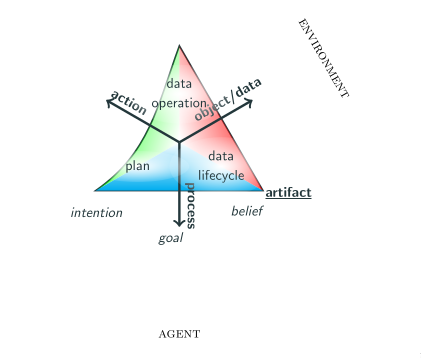
\includegraphics[scale=0.7]{01/ao.png}
  \caption{Forze nel paradigma Agent-oriented.}
\end{figure}

\qs{}{Come realizzare agenti intelligenti? Come costruire agenti che abbiano le caratteristiche di autonomia, di reattività, di proattività e di abilità sociali fin qui citate?}

\begin{itemize}
  \item 1956-1985: la maggior parte dei progetti di architetture per agenti si basano sul \fancyglitter{ragionamento simbolico} sviluppato per IA. Utilizzo del ragionamento logico per capire cosa fare. 
  \item 1985-presente: \fancyglitter{Reactive agents movements}. 
  \item 1990-presente: \fancyglitter{architetture ibride} che combinano il meglio delle architetture basate sul ragionamento logico e quelle reattive. (e. g. Jason).
\end{itemize}

\nt{Il classico approccio per costruire agenti intelligenti è quello di vederli come casi particolari di sistemi basati sulla conoscenza (paradigma \fancyglitter{symbolic AI}).}

\paragraph{L'architettura di un agente deliberativo:}

\begin{itemize}
  \item Contiene una esplicita rappresentazione (\fancyglitter{modello simbolico}) dell'ambiente. 
  \item Prende decisioni attraverso un \fancyglitter{ragionamento simbolico}.
\end{itemize}

\paragraph{Però ci sono due problemi da affrontare:}

\begin{itemize}
  \item \fancyglitter{Il problema della trasduzione}: il problema della traduzione del mondo reale, dell'ambiente, in una descrizione simbolica accurata, in tempo perché possa essere utile.
  \item \fancyglitter{Il problema della rappresentazione/ragionamento}: il problema di come rappresentare simbolicamente le informazioni su entità e processi complessi del mondo reale, e come fare in modo che gli agenti ragionano con queste informazioni in tempo perché i risultati possano essere utili.
\end{itemize}

\clm{}{}{
  \begin{itemize}
    \item Entrambi i problemi non sembrano facilmente risolvibili, servono alternative. 
    \item Il problema risiede nella \fancyglitter{complessità} degli algoritmi di manipolazione simbolica. La maggior parte degli algoritmi rilevanti sono \fancyglitter{altamente intrattabili}. 
  \end{itemize}
}

